\section{Frozen noisy-recovery and rejection study}
\label{app:trusted-experiments}

\paragraph{Prospective splits and observations.}
The local protocol and source freeze are
\texttt{research/TRUSTED\_RECOVERY\_PROTOCOL.md} and
\texttt{research/TRUSTED\_RECOVERY\_FREEZE.json}.
They are timestamped execution records, not an independent preregistration.
Development uses synthetic seeds 0--3 and existing byte-LM seed 10.
Calibration uses synthetic seeds 100--119 and newly trained byte-LM seeds
20--21; evaluation uses synthetic seeds 200--239 and new byte-LM seeds
22--25. The six fresh checkpoints use the unchanged width-128, $L=12$,
$K=4$, 6000-step configuration of the preceding controlled training study.
There is no checkpoint selection on recovery outcomes.

Synthetic factors have $L=6,K=3,D=16$, random-normal bases, and four router
regimes: interior softmax, contractions toward the uniform router by factors
$0.1$ and $0.01$, and a contraction toward balanced one-hot rows by $0.01$.
Each instance supplies 16 normalized Gaussian gradient directions.
Language directions are actual effective-parameter cross-entropy gradients
from 16 training-split minibatches of size $2\times32$, sampled with fixed
seed offset 3100000. Four or twelve initial directions fit the estimator;
the last four assess held-out response fit. Response observations come from
automatic differentiation of the factor map, without calling its closed-form
response formula.

Product and each response receive independently drawn Gaussian perturbation
directions rescaled to relative Frobenius norms
$\sigma\in\{0,10^{-8},10^{-6},10^{-4},10^{-3},10^{-2}\}$.
Directions are shared across noise levels within an instance.
The supplied bound $\sigma$ is known; the true perturbation vector and factors
are not supplied to recovery. The estimated rank-$K$ product row subspace
is used by all methods, and evaluation includes basis error outside it.
This observation-noise experiment does not model biased, adversarial,
quantized, or unknown optimizer-state errors.

\paragraph{Fixed estimators and observable scores.}
The projected spectral baseline clips router entries below $10^{-8}$,
normalizes rows, and refits the basis by least squares. Joint fitting uses
simplex logits in orthonormal zero-sum coordinates and normalized basis
coordinates, with SciPy trust-region reflective least squares and exact
forward-mode Jacobians. Three starts are fixed: projected spectral,
a $0.1$ logit perturbation, and a random simplex router. Each has a budget
of 80 function evaluations; the smallest observed training residual selects
the output. There is one developed solver variant, with no tuning on
calibration or evaluation factors.

All acceptance rules require a numerically feasible router and finite score.
The combined score is the maximum of (i) training plus held-out residual
plus twice the normalized noise budget, divided by the simplex-tangent
Jacobian's smallest singular value; (ii) an observed product-subspace
perturbation ratio; and (iii) permutation-aligned disagreement among
competitive starts for the joint fit. A separately disclosed $10^{-10}$
numerical floor enters the empirical noise budget.
The comparison scores use only residual or inverse Jacobian singular value.
Their implementation and thresholds are frozen, and no score uses truth
at prediction time.

For each method/score pair, one threshold is chosen on pooled calibration
data to maximize accepted count, subject to at least 20 accepted synthetic
outputs and at most $5\%$ bad among all accepted outputs. Ties are accepted
together. An infeasible threshold would reject all and be reported as a
failure. The same threshold transfers to both evaluation domains.
Good errors are at most $0.05$, bad errors exceed $0.10$, and intermediate
errors are reported separately. This empirical calibration is not a
distribution-free risk guarantee.

\begin{table}[t]
\centering
\small
\caption{Synthetic held-out diagnostic comparison (percent). Coverage is the accepted fraction; bad rejection is recall on errors $>0.10$; good rejection is false rejection on errors $\le0.05$; accepted bad is the bad fraction among accepted outputs. Each threshold was frozen using calibration only.}
\label{tab:trusted-diagnostics}
\begin{tabular}{llrrrr}
\toprule
Method & Score & Coverage & Bad reject & Good reject & Accepted bad \\
\midrule
Spectral & Combined & 10.21 & 100.00 & 85.04 & 0.00 \\
Spectral & Residual & 10.21 & 100.00 & 85.04 & 0.00 \\
Spectral & Condition & 10.26 & 100.00 & 84.96 & 0.00 \\
Projected & Combined & 72.71 & 90.11 & 0.00 & 4.01 \\
Projected & Residual & 72.66 & 92.23 & 0.00 & 3.15 \\
Projected & Condition & 21.30 & 98.06 & 70.48 & 2.69 \\
Joint fit & Combined & 92.81 & 59.47 & 0.18 & 5.16 \\
Joint fit & Residual & 91.51 & 70.04 & 0.18 & 3.87 \\
Joint fit & Condition & 24.32 & 91.63 & 72.73 & 4.07 \\
\bottomrule
\end{tabular}
\end{table}


\paragraph{Results, including unsuccessful diagnostics.}
All 1920 synthetic joint fits return; there are 1639 good, 54 intermediate,
and 227 bad outputs. Projected spectral recovery has three failed outputs,
all retained in the 1920-case denominator.
Seventy selected joint-fit runs exhaust their 80-evaluation budget; a returned
estimate is not a convergence claim. Competitive-start agreement is also
not a uniqueness test, especially if only one start meets the residual cutoff.
Joint fitting improves error in 1916 of the 1917 paired successful
synthetic comparisons and all 48 language comparisons.
This comparison counts correlated variants, not independent replications.

The combined joint-fit diagnostic rejects $59.47\%$ of bad synthetic
outputs, with $0.18\%$ false rejection of good outputs and $92.81\%$
coverage. Seed-cluster bootstrap 95\% intervals, resampling the 40 independent
seeds and retaining all their variants, are respectively
$[54.79\%,63.82\%]$, $[0,0.49\%]$, and $[92.08\%,93.54\%]$.
Residual-only rejection instead rejects $70.04\%$ of bad outputs with
the same good false-rejection rate, at $91.51\%$ coverage.
Condition-only rejection discards $72.73\%$ of good outputs.
The raw spectral method's feasibility gate rejects almost all noisy
candidates: its high rejection recall is not useful broad coverage.

Failures concentrate near router rank collapse.
At contraction $0.01$, joint fitting has $165/480$ bad outputs; the combined
score accepts 352, including 37 bad outputs. At contraction $0.1$, it accepts
473 of 480, including 55 bad outputs. Thus aggregate calibration masks
substantial regime-specific error rates. Interior and near-boundary
regimes have no errors above $0.10$ on this grid.
The largest joint-fit error is $10.54$; the largest falsely accepted error,
$0.820$, occurs at seed 210, contraction $0.01$, $\sigma=10^{-3}$, $q=4$.
These cases remain in the released records and were not used to retune
the primary thresholds.

All 48 language joint fits are good and accepted. Maximum error at seeds
22, 23, 24, and 25 is respectively $0.00752$, $0.01063$, $0.01002$,
and $0.00650$. There are only four independent training runs, and no bad
joint-fit output in this cohort: bad-output rejection recall is undefined,
not demonstrated to be perfect.
The projected baseline has one bad language output and accepts it.
The condition-only joint-fit rule rejects every language output.
An all-reject outcome is explicitly uninformative.

\begin{figure}[t]
\centering
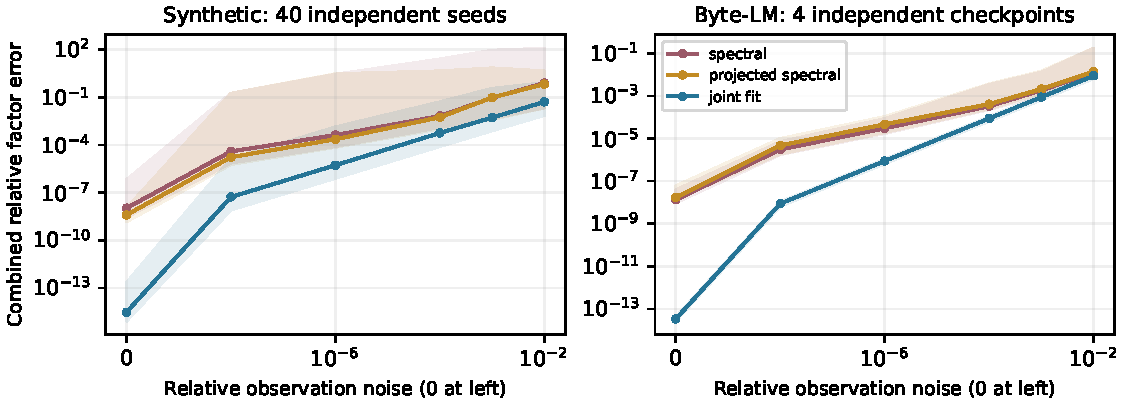
\includegraphics[width=\linewidth]{figures/trusted_recovery.pdf}
\caption{Held-out recovery under simultaneous product and response noise.
Lines show medians and shading the 10th--90th percentiles of the fixed grid,
not confidence intervals. Synthetic aggregation includes all four regimes
and both probe counts; language aggregation includes four checkpoints and
both probe counts. Zero noise is placed at the leftmost plotting coordinate.
Tail failures and diagnostic errors are reported separately.}
\label{fig:trusted-recovery}
\end{figure}

\paragraph{Numerical local separation and reproducibility.}
The 140 synthetic local passes occur in the interior (60) and near-boundary
(80) regimes; there are none in the two rank-contracted regimes.
Only two language outputs pass, both at seed 22.
The pass concerns an estimated-subspace feasible component and has no
unconditional truth-error interpretation.
Raw observations, estimates, starts, failures, diagnostics, source hashes,
calibration thresholds, and per-seed summaries are released under
\texttt{results/trusted\_recovery/}.
Full-coordinate theorem checks are distinct from the recovery experiment.
A separate CPU environment replays the frozen observations; its results
are recorded separately because floating-point optimization need not be
bitwise identical. Across all 1968 cases, good/intermediate/bad classifications
agree for every method. Combined-score acceptance changes in four spectral
and two joint-fit cases; the largest joint-fit error difference is $0.0171$.
Thus environment agreement is assessed explicitly, not inferred from tests.
The release verification rebuilds the reported tables
and checks source and threshold bindings.
